\documentclass{bmstu}


\usepackage{physics}
\usepackage{pdfpages}
\usepackage{tabularx}
\usepackage{longtable}
\usepackage{xfrac}
\usepackage{amssymb}
\usepackage{dsfont}
\usepackage{upgreek}
\usepackage{color, colortbl}
\usepackage{listings}
\usepackage{ amssymb }
\usepackage{tikz}

\graphicspath{
	{graphics/}
}

\begin{document}
	
	\section*{20/09}
	
	\begin{center}
		\textbf{Хранение разреженных матриц}
	\end{center}
	
		\underline{Опр.} Портретом разреженной матрицы называется множество:
		\[
		P_A=\{(i,j):a_{ij}\neq0\}
		\]
		
		\begin{enumerate}
			\item Матрица несимметрична и ее портрет несимметричен:
			\[
			\exists \ (i, j) \in P_A: (j, i) \notin P_A \Leftrightarrow A\neq A^{\text{Т}}
			\]
			\[
			\begin{bmatrix}
				1&2 \\ 0&0
			\end{bmatrix}
			\Rightarrow 
			\begin{bmatrix}
				\ast&\ast \\ 0&0
			\end{bmatrix}
			\]
			\item Матрица несимметрична но её портрет симметричен:
			\[
			A\neq A^{\text{Т}}, \text{ но } (i, j) \in P_A, (j, i) \in P_A, a_{ij}\neq a_{ij}
			\]
			\[
			\begin{bmatrix}
				1&0 \\ 0&2
			\end{bmatrix}
			\Rightarrow 
			\begin{bmatrix}
				\ast&0 \\ 0&\ast
			\end{bmatrix}
			\]
			\item Если матрица симметрична ($a_{ji}=a_{ij}$), то её портрет симметричен:
			\[
			\begin{bmatrix}
				1&0 \\ 0&1
			\end{bmatrix}
			\Rightarrow 
			\begin{bmatrix}
				\ast&0 \\ 0&\ast
			\end{bmatrix}
			\]
		\end{enumerate}
		
\underline{CSR} - compressed sparse row

\underline{CSC} - compressed sparse column

\underline{CSLR} - compressed sparse low triangle (почему R)

\begin{enumerate}
	\item aelem - массив, хранящий все $a_{ij}\neq 0$ в строках
	\item jptr - размерность aelem, указывает $N_j$ элемента $a_{ij}$
	\item iptr - размерность $n+1$ ($n$ - размерность СЛАУ), хранит число элементов $a_{ij}\neq 0$ в строке
	
	iptr$[i+1]$ - iptr$[i]$ - число элементов в i-ой строке
	iptr$[n+1]$ - число элементов в aelem + 1
	\item adiag - все диагональные элементы
	\item altr - элементы нижнего треугольника
\end{enumerate}

\underline{Пример:}
\[
A=
\begin{bmatrix}
	9&0&0&3&1&0&1 \\
	0&11&2&1&0&0&2 \\
	0&1&10&2&0&0&0 \\
	2&1&2&9&1&0&0 \\
	1&0&0&1&12&0&1 \\
	0&0&0&0&0&8&0 \\
	2&2&0&0&3&0&8 
\end{bmatrix}
\]

Матрица $A$ несимметрична, а $P_A$ симметричен, т.к. если $a_{ij}\neq 0$, то $a_{ji}\neq 0$.

aelem: $\left[\left[ 9, 3, 1, 1 \right], \left[11, 2, 1, 2\right], \left[1, 10, 2\right],\left[2, 1, 2 ,9, 1\right],\left[1, 1, 12, 1\right],\left[8\right],\left[2, 2, 3, 8\right] \right]$.

jptr: $\left[\left[1, 4, 5, 7\right], \left[2, 3, 4, 7\right], \left[2, 3, 4\right],\left[1, 2, 3, 4, 5\right],\left[1, 4, 5, 7 \right],\left[6\right],\left[1, 2, 5, 7\right] \right]$.

iptr: $\left[1, 5, 9, 12, 17, 21, 22, 26\right]$.

adiag: $\left[9, 11, 10, 9, 12, 8, 8\right]$.

altr: $\left[1,2, 1, 2, 1, 1, 2, 2, 3\right]$.

Если матрица несимметричка, то храним ещё и элементы нижнего треугольника, но уже по столбцам (для сохранения структуры).

К ЧЕМУ ЭТО

autr: $\left[2, 3, 1, 2, 1, 1, 1, 2, 1\right]$.

jptr: $\left[2, 1, 2, 3, 1, 4, 1, 2, 5\right]$.

iptr: $\left[1, 1, 1, 2, 5, 7, 7, 10\right]$.

Я НЕ ПОНИМАЮ

Входные данные: $\overline{x}$, aelem, jptr, iptr, n.
\[
z = A\overline{x}, \ A - CSR
\]

как оформить код (а главное, зачем в нем столько скобок) - а хуй его знает

\newpage
	\begin{center}
	\textbf{Учет граничных условий}
\end{center}

\underline{Граничные условия I рода}

Зададим температуру в узле $a_{33}$:
\[
A=\begin{bmatrix}
	\cdots & &\cdots & &\cdots  \\
	\cdots & 0 & 1 & 0 & \cdots \\
	\cdots & &\cdots & &\cdots 
\end{bmatrix}
\]

Чтобы не испортилась симметричность портрета, искусственно обнулим необходимые элементы массива aelem.  

(я не понимаю к чему относится часть первой строки в коде после точки с запятой)

\begin{lstlisting}
	i = iptr[k]; iptr[k+1]-1
	{ 
		if jptr[i=k]
			aelem[jptr[k]]=1;
		else
			aelem[jptr[k]]=0;
	}
\end{lstlisting}

\underline{Метод Холецкого}
\[ \begin{matrix}
	A\approx LU\\A = LU+R
\end{matrix}
\]

где $L$ - нижнетреугольная матрица;\\
\hangindent=2.05cm
$U$ - верхнетреугольная матрица;\\
	$R$ - ошибка округления.
	
	\[
	\begin{cases}
		Ax= b \\ LUx= b \\ Ly = b \Rightarrow Ux=y
	\end{cases}
	\]
	
	\newpage
	\begin{center}
		\textbf{Предобусловливание}
	\end{center}
	
	Число обусловленности: $\frac{\lambda_{min}}{\lambda_{max}}<1$
	
	Так оно меньше единицы или больше?
	\begin{figure}[h]
		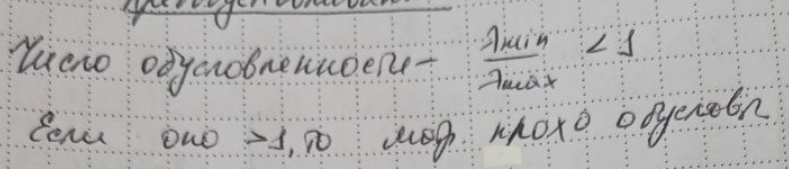
\includegraphics[height=0.2\linewidth]{уааа.png}
	\end{figure}
	
	M - матрица предобусловливания
	
	\begin{enumerate}
		\item M должна быть по возможности близка к A (пример: M = diag(A)).
		\item M должна быть легко вычислима.
		\item M должна быть обратима.
	\end{enumerate}
\end{document}